\section{Methodology} \locallabel{sec:methodology}

In this section we describe the classes in our study, the concept of a feedback
delay, and provide some details on our system architecture.

\subsection{Classes}

\begin{figure}[!t]
\centering \includegraphics[width=3.3in]{graphs/Class_Information.eps}
\caption{The numbers of groups, students, and average number of submissions by
  student for each of the seven classes in the study.}
\locallabel{fig:class_info}
\end{figure}

Our study involves multiple instances of two courses. The first course,
\emph{CS24}, is the second required course in UCSB's lower division Computer
Science curriculum that builds upon student's prior knowledge of \emph{C} in
order to educate them on basic data structures, and basic object oriented
programming in \emph{C++}. The second course, \emph{CS64}, is a lower division
computer architecture course that educates students on assembly programming and
the basics of computer architecture including digital design. In total, there
are five instances of \emph{CS24}, and two instances of \emph{CS64} represented
in this study. \cm[24]{13} and \cf[24]{13} were taught by a single instructor,
and the remainder we taught by another instructor. All classes were taught
during a 10-week quarter including the summer instance.

Figure~\localref{fig:class_info} shows the relevant information for each of the
classes in this study. The purple bars indicate the number of students who
provided consent in each of the classes. The cyan bars indicate the number of
unique groups to make submissions on the class's assignments, and the pink bars
indicate the average number of submissions made by each student. Submissions
for non-programming assignments are excluded.

We distinguish between students and groups because the submission system
supports an instructor defined group size on a per assignment basis allowing
students to manually form groups for such assignments. Where groups are
concerned, only submissions for which we have the consent of all group members
are included. This grouping functionality was only introduced in September,
2014, and thus it was only utilized in classes \cf[24]{13} and \cw[24]{14}. In
those classes, the groups did not remain consistent as students could change
partners, or chose to work independently (considered a single student group)
from assignment to assignment.

The average number of submissions is low for \cw[24]{13} due to only using the
submission system for half of the quarter. The average number of submissions
per student for \cm[24]{13} is relatively high due to students making
post-deadline submissions as discussed in section~\localref{sec:deadline}.


\subsection{Feedback Delay}
\locallabel{sec:delay}
The purpose of the real-time feedback system is simply to provide feedback to
the students so they may iteratively achieve mastery of an assignment. The
usage of such systems has positive side effects including reducing assessment
time while increasing assessment equitability. However, as many have previously
observed, student usage of such systems may result in dependency upon the
system. This dependency could inhibit students from expanding their knowledge
of the compilation, execution, testing and debugging processes.

Web-CAT ensures students develop testing skills by requiring students to submit
test cases along with their code~\cite{Edwards:2003:RCS:949344.949390}. While
this approach appears successful to help students develop testing skills, such
an approach would require a change to our lower-division curriculum. In order
to encourage students to start assignments earlier, Marmoset introduced the
concept of limited release tokens where feedback from a subset of tests could
only be received a few times a day. In theory, the release token approach
should also discourage dependency on the system, however, in practice \spacco{}
indicated that very few students took advantage of the release
tokens~\cite{Spacco:2013:TIP:2462476.2465594}.

We built our system in order to take an alternative approach that could
transparently be utilized by UCSB's CS curriculum. Our approach is to introduce
a configurable per-assignment delay between the time that students can receive
new feedback. For example, if the delay is configured as five minutes, that
means students can receive feedback from only one new submission in any five
minute window. Alternatively, if students make submissions exactly five minutes
or more apart, they will never experience any delays in receiving feedback. Our
hypothesis was that as the delay increased, students would spend more time
testing their assignment prior to submission and the result would be both an
increased time between submission, and an improvement in submission efficiency.

In attempt to measure effects on the feedback delay, three of our classes
increased the feedback delay in five minute increments for each subsequent
assignment. Those classes were \cs[24]{13}, \cm[24]{13}, and \cf[24]{13}. In
all other classes the delay was not intentionally altered between
assignments. The impact of the delay is covered in
section~\localref{sec:sub_impact} and section~\localref{sec:session_impact}.


\subsection{System Architecture}

\begin{figure}[!t]
\centering 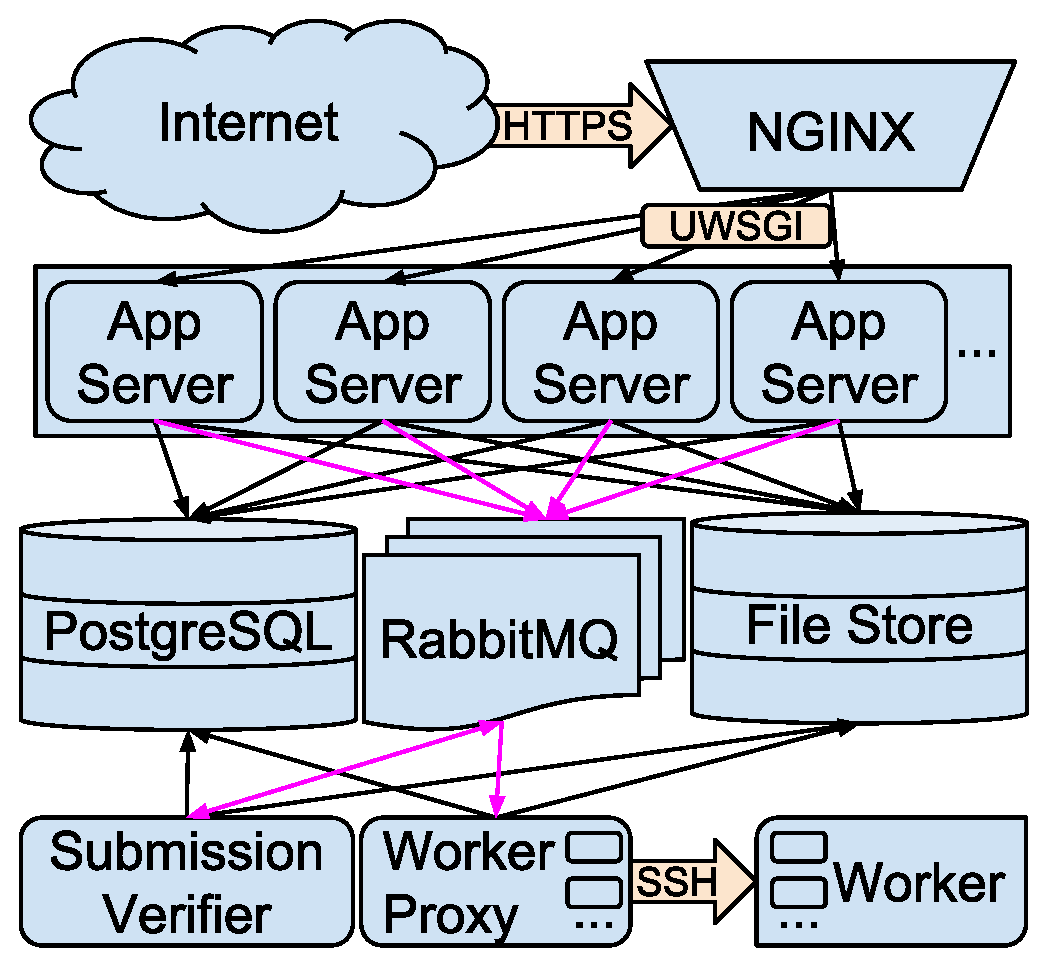
\includegraphics[width=3.3in]{graphs/architecture.eps}
\caption{An overview of the system architecture and how components
  interact. Pink lines indicate messages being passed to and from the RabbitMQ
  service. Note that each \emph{Worker} runs in a separate isolated
  environment.}
\locallabel{fig:architecture}
\end{figure}

We designed our real-time submission and feedback system with security and
ease-of-use in mind. There are three primary components to the system
architecture:

\begin{description}
\item[back-end] Exposes the API allowing instructors and/or teaching assistants
  to create and configure assignments, view student submissions and aggregate
  scores; and allowing students to make submissions to assignments and view the
  associated feedback
\item[front-ends] Provides the interface for which instructors and students
  interact with the submission system. A \emph{html5} Bootstrap template
  provides the primary interface through a web browser, though command line
  programs are also used and convenient for submitting assignments and
  batch-uploading assignment test cases.
\item[workers] Verifies, compiles, and executes the students' untrusted code
  against each test case and compares the results to the expected.
\end{description}

Figure~\localref{fig:architecture} provides a diagram of the overall
architecture. At present all of the components save for each \emph{Worker} run
on a single machine as we have not run into any web service related performance
issues. We describe each component in the following subsections.

\subsubsection{Back-End}
The back-end provides a REST-API which was built using the python-based Pyramid
Web Framework. Python was chosen as the language due to the author's experience
with the language thus allowing rapid deployment and modifications to the
system.

NGINX, an event-based webserver, handles HTTPS connections and distributes
requests to an instance of the Pyramid application via UWSGI. The individual
applications can each read from and write to both the file store and the
PostgreSQL database, and create \emph{validate submission} jobs via the
RabbitMQ messaging service. The database stores all of the \emph{user},
\emph{class}, \emph{assignment}, and \emph{submission} meta-data. The file
store saves all uploaded files which includes files belonging to submissions,
test case input and expected output, pre-rendered html-diff output between test
case output and actual output produced by submitted programs, and a few other
files an instructor may associate with an assignment. Files are stored by
sha1sum so that duplicate files only require additional meta-data.

The REST-API supports the following common actions with the associated
permissions:

\begin{itemize}
\item account creation (requires UCSB email)
\item class creation (administrators)
\item class manager addition (administrators and class managers)
\item assignment creation (associated class managers)
\item assignment modification (associated class managers)
\item file creation (authenticated users)
\item file view (associated authenticated users)
\item submission creation (associated class managers and associated class
  members)
\item submission view (class managers associated with the class, and
  authenticated users associated with the submission
\end{itemize}

Additional API actions allow students to make group requests, and confirm or
deny those requests. Furthermore, a significant subset of API actions pertain
to assignment configuration, however, we will not detail the specifics of
project configuration.

\subsubsection{Front-Ends}
The primary interface to the system is via a web browser through an easy-to-use
HTML5 interface based on the popular Bootstrap front-end web framework. The web
interface supports all of the API functions, most importantly by providing
drag-and-drop submission creation.

Because of the REST API provided by the back-end, any number of additional
front-end interfaces can easily be written by students or instructors. All data
is sent over the HTTP protocol and encoded via JSON. Of note are two command
line interfaces written to help expedite some of the system work flows:

\begin{itemize}
\item A submission creation program was written, which authorizes the student
  and creates a submission by first uploading the submission files, and then
  associating those IDs with a new submission. The student is immediately
  provided a link where they can receive feedback.\footnote{Feedback is
    currently only accessible via the web interface.}
\item An assignment test case synchronization program was written, which allows
  an \emph{class manager} to quickly synchronize an assignment on the system
  with the contents of a directory on their local system. This program can
  dramatically decrease the time to configure and an assignment because while
  it is easy to add test cases, it can be tedious if there are more than a
  handful of them. Moreover, while this program expects the test cases to be
  provided in a certain format, it would be trivial to alter the program for
  another format.
\end{itemize}

\subsubsection{Workers}
The system makes use of three classes of workers. The first is responsible for
verifying submissions. When a submission is made by a student, the receiving
\emph{application server} creates a \emph{validate submission} job. When
notified of a job, a \emph{Submission Verifier} worker verifies the necessary
files were submitted and that each file passes inspection. A file may not pass
inspection if it is too large, too small, or contains invalid content as
specified by a regular expression. If the submission passes verification a
\emph{test executable} job is created for each executable configured for the
assignment by a \emph{class manager}.

The \emph{Worker Proxy} workers are notified of \emph{test executable} jobs and
are responsible for interfacing with the external simply named \emph{Worker}
workers. There is a one-to-one mapping between a \emph{Worker Proxy} and the
account that the \emph{Worker} it interfaces with uses. The \emph{Worker Proxy}
performs the following actions in order:

\begin{enumerate}
\item select a lab machine to run on
\item force kill any processes that may be running as the worker user on the
  chosen machine
\item prepare a directory with all files necessary to build and execute the
  submission with the necessary test case inputs
\item \emph{rsync} the directory to the remote machine
\item execute the \emph{Worker} process via \emph{ssh} (see to next paragraph)
\item fetch the test case output files and execution meta-data via \emph{rsync}
\item generate and store the results from the submission's execution
\end{enumerate}

As the previous list indicates a \emph{Worker} is invoked via \emph{ssh}. The
machines these workers run on are the same machines the students use to test
their programs thus providing a testing environment consistent with the
development environment. The accounts used for testing only ever test a single
project at a time and clean up the environment when completed. Furthermore, the
worker accounts have network access restricted via an \emph{iptables} rule so
that no network connections may be established. While this setup does not
prevent students from leaking assignment data to world-writable directories,
doing so would be a punishable abuse of the system. Regardless, the worst a
student could do is extract test case inputs and alter test case execution
meta-data. However, test case inputs can be leaked through the feedback system
with clever output encoding and multiple submissions (the feedback is limited
intentionally to make this nontrivial), and the \emph{Worker Proxy} treats the
meta-data and files it fetches as untrusted. Moreover altering the meta-data
can only result in the failing of a test case. It is important to note that
test case expected output is never sent to a \emph{Worker}.
